\documentclass[preprint,12pt,number,sort&compress]{elsarticle}
\usepackage[a4paper,margin=1in]{geometry}
\usepackage[T1]{fontenc}
\usepackage{microtype}
\usepackage{amsmath,amssymb,mathtools,amsthm}
\let\openbox\relax
\usepackage{txfonts}
\usepackage{booktabs,tabularx,array,longtable,multirow,threeparttable}
\usepackage{graphicx,adjustbox,xcolor,xspace,enumitem,caption,needspace,setspace,seqsplit}
\usepackage{hyperref}
\usepackage{xurl}
\journal{Knowledge-Based Systems}
% Identity facts are confirmed; this switch does not certify final submission approval.
\newif\ifAuthorFactsConfirmed
\AuthorFactsConfirmedtrue
\newcommand{\AuthorList}{Runze Zhu, Guanfeng Li}
\newcommand{\AffiliationBlock}{School of Information Engineering, Ningxia University, Yinchuan, China}
\newcommand{\AuthorContributions}{\textbf{Runze Zhu:} Conceptualization, Methodology, Software, Data curation, Investigation, Validation, Writing -- original draft. \textbf{Guanfeng Li:} Writing -- review and editing, Formal analysis, Supervision.}
\newcommand{\FundingStatement}{This work was supported by the Natural Science Foundation of Ningxia (Grant No. 2026AAC020029) and the National Natural Science Foundation of China (Grant No. 62066038).}
\newcommand{\CompetingInterests}{The authors declare no relevant financial or non-financial competing interests.}

\providecommand{\PaperTitle}{PAIR: Verifiable quantitative knowledge and model comparison from incomplete experimental references}
\providecommand{\PlainAuthors}{Runze Zhu; Guanfeng Li}
\hypersetup{hidelinks,pdfauthor={\PlainAuthors},pdftitle={\PaperTitle}}
\newtheorem{theorem}{Theorem}
\newtheorem{proposition}{Proposition}
\newtheorem{corollary}{Corollary}
\newtheorem{definition}{Definition}
\newtheorem{remark}{Remark}
\newcommand{\method}{PAIR\xspace}
\newcommand{\pairkg}{PAIR-KG\xspace}
\newcommand{\paireval}{PAIR-Eval\xspace}
\newcommand{\compiler}{PAIR-Compile\xspace}
\newcommand{\R}{\mathbb{R}}
\DeclareMathOperator{\rank}{rank}
\DeclareMathOperator{\col}{col}
\DeclareMathOperator{\row}{row}
\DeclareMathOperator{\nnz}{nnz}
\setstretch{1.10}
\setlength{\parindent}{1em}
\setlength{\parskip}{0pt}
\setlength{\emergencystretch}{2em}
\renewcommand{\arraystretch}{1.15}
\newcolumntype{L}[1]{>{\raggedright\arraybackslash}p{#1}}
\renewcommand{\tabularxcolumn}[1]{>{\raggedright\arraybackslash}p{#1}}
\captionsetup{font=small,labelfont=bf,skip=8pt}
\setlist{nosep,leftmargin=*}
\raggedbottom
\renewcommand{\topfraction}{0.92}
\renewcommand{\textfraction}{0.08}
\renewcommand{\floatpagefraction}{0.85}
\makeatletter
\setlength{\@fptop}{0pt}
\setlength{\@fpsep}{16pt}
\setlength{\@fpbot}{0pt plus 1fil}
\makeatother

\begin{document}
\begin{frontmatter}
\title{\PaperTitle}
% Identity and affiliation facts restored from the 2026-11-03 Paper2 R7 author-review source, with user authorization.
\author[aff1]{Runze Zhu}
\ead{zhurunze44@gmail.com}
\author[aff1]{Guanfeng Li\corref{cor1}}
\ead{ligf@nxu.edu.cn}
\cortext[cor1]{Corresponding author.}
\address[aff1]{School of Information Engineering, Ningxia University, Yinchuan, China}

\begin{abstract}
Knowledge-based systems need quantitative assertions whose numerical meaning remains valid when experimental references are incomplete. We introduce PAIR (Projection-Aligned Identifiable Relations), connecting verifiable knowledge compilation with model comparison through a shared reference geometry. PAIR-KG retains complete linear comparisons, binds them to a registered completion and local witness, and verifies reference estimability and declared shared-source cancellation. Its properties include aggregation closure, source-refinement monotonicity, universal completion conditions and explicit operator-application costs. PAIR-Eval uses the dual quotient space to separate resolved prediction error from training-unresolved offsets and characterize model-order invariance under truth-only completion shifts, including three-way preferences on bounded domains. K562 and ENCODE retain 2,635 (26.50\%) and 56,395 (5.79\%) compound-only dimensions beyond individually estimable effects. Replogle metadata establish shared-control cancellation for 100,000 registered four-cell designs. For seven fixed CTRPv2 predictors on registered model-specific supports, full-to-resolved scoring reverses median fractions of 50.0\% of model-pair orders under normalized $R^2$ and 35.7\% under normalized Pearson correlation, with five persistent pair--metric reversals. GDSC2 exhibits 30.0\% median fold-level reversals; persistence checks distinguish target sensitivity from recurring model preferences. PAIR preserves the comparative information needed to verify quantitative knowledge and interpret predictive decisions.

\end{abstract}
\begin{keyword}
Quantitative knowledge representation \sep Knowledge verification \sep Incomplete experimental references \sep Data provenance \sep Quotient-space model evaluation \sep Three-way decisions
\end{keyword}
\end{frontmatter}

\section{Introduction}\label{sec:intro}
Knowledge-based systems turn experimental evidence into reusable assertions and predictive decisions. A quantitative assertion must preserve what was compared, the reference used to adjust the measurements, and the sources that contribute to its value. These requirements matter when measurements cover only part of a multi-factor experiment: a reference may determine a comparison among several measured cells while leaving each adjusted cell individually underdetermined. The same distinction affects model selection, because scoring a predictor on unresolved reference components can change which model appears preferable.

Molecular perturbation screens provide a concrete setting. A response at regulator--event coordinate $(r,e)$ combines regulator-wide activity, event-specific sensitivity, technical or control offsets, and pair-specific interaction~\cite{tian2017apa,kowalski2024cpa}. A balanced four-cell difference-in-differences comparison cancels additive regulator and event effects. For sparse, overlapping designs, more general comparisons require the actual training reference $X_R$ to determine whether the corresponding baseline contribution is estimable. The evaluation responses $Y_E$ are measured; the incompleteness concerns the reference used to interpret them.

Evidence-based knowledge graphs preserve source material and support traceable reuse~\cite{hogan2021knowledge,unni2022biolink}. Recent systems link claims to supporting literature and retain conflicting findings~\cite{shamshiri2026security}; biomedical graph enrichment also combines retrieval, schema alignment and relation validation with explicit provenance~\cite{mohamed2026orchestra}. For a relation computed from several measurements, the additional question is numerical: do the declared reference and shared-source terms cancel in the reported comparison? Detaching the value from its signed coefficients or completion rule prevents that question from being checked. Symbolic lineage~\cite{green2007provenance,w3c2013prov,sen2026provsql} supplies dependencies; algebraic verification supplies the cancellation test.

Predictive benchmarks encounter the same reference geometry. In leave-drug-out pharmacogenomics~\cite{bernett2026dreval}, a training reference can identify relative response profiles without identifying an unseen drug's overall offset. Ambient scoring combines these components, whereas a reference-resolved target retains the identified profile. Matrix imputation~\cite{mazumder2010softimpute,vo2026pica} supplies completed values under reconstruction assumptions; estimability theory~\cite{searle1971linear,rao1971generalized} determines which comparisons already follow from the reference. Decision methods for incomplete information~\cite{li2026clustering,li2026incomplete,zhang2026adaptive} further motivate distinguishing supported decisions from boundary cases.

We ask: \emph{Which quantitative comparisons does an incomplete experimental reference support, and how can a knowledge system preserve that information when compiling assertions and comparing predictive models?} We propose \textbf{\method} (\textbf{P}rojection-Aligned \textbf{I}dentifiable \textbf{R}elations), with two interfaces sharing the coefficient--response duality $\ker(U^\top)=\operatorname{range}(Q)$ (Fig.~\ref{fig:overview}). Its contributions are:
\begin{enumerate}
\item \textbf{A reference-bound representation for quantitative knowledge.} \pairkg retains each complete comparison $(a,h,z_{F_R}(a))$, binding its coefficients to a registered completion and a local witness. Reference and source gates distinguish qualified assertions, measurement records and refusals.
\item \textbf{Verifiable compilation properties.} Building on classical estimability, we establish four local witness identities and aggregation closure (Proposition~\ref{prop:soundness}), source-refinement monotonicity (Corollary~\ref{cor:refinement}), and universal completion conditions for balanced four-cell contrasts (Proposition~\ref{prop:fourcell}). The computational analysis includes the registered completion operator's application cost.
\item \textbf{Reference-resolved model comparison.} \paireval scores the dual quotient response space, decomposes prediction error and characterizes model-order invariance under truth-only completion shifts (Proposition~\ref{prop:order}). Bounded completion domains support strict preferences for either model or a boundary decision.
\item \textbf{Comparative evidence across molecular and drug-response resources.} We quantify compound information retention, reference and source verification, and ranking consequences across four perturbation resources and three pharmacogenomic cohorts. Fixed-prediction scoring and persistence controls distinguish evaluation-target sensitivity from model preferences that recur across folds and resources.
\end{enumerate}

Section~\ref{sec:related} reviews related work. Sections~\ref{sec:problem} and~\ref{sec:framework} define the problem and framework, Sections~\ref{sec:design} and~\ref{sec:results} present the evaluation, and Sections~\ref{sec:discussion} and~\ref{sec:conclusion} discuss the findings and conclude.

\section{Related work}\label{sec:related}
\method connects quantitative knowledge representation, estimability under incomplete references and model decisions under partial information. Table~\ref{tab:paradigms} compares their input objects and verification contracts.

\begin{table}[t]
\centering\small\setstretch{1.05}
\caption{Architectural comparison of information-processing paradigms under incomplete reference designs. Comparisons reflect the mathematical objects and guarantees defined by each paradigm.}
\label{tab:paradigms}
\begin{tabularx}{\textwidth}{@{}L{0.16\textwidth}XXXX@{}}
\toprule
Dimension & Matrix Completion \& Imputation & KG Reification \& Provenance & Ambient Benchmark Scoring (\texttt{FULL}) & \textbf{\method (\pairkg + \paireval)} \\\midrule
Fundamental information granule & Reconstructed atomic cell entries $\widehat{Y}_{re}$ & Symbolic triples, semantic units, or lineage polynomials & Ambient held-out response vector $y \in \R^{n_E}$ & Contrast tuple $(a, h, z_{F_R}(a))$ and quotient response $Qy$ \\
Treatment of rank-deficient $X_R$ & Imposes low-rank spectral or distributional priors & Schema-level representation without rank checks & Scores resolved and unresolved subspaces jointly & Exact orthogonal decomposition $\operatorname{range}(Q) \oplus \col(U)$ \\
Completion \& verification contract & Implicitly defined by fitted reconstruction solver & Symbolic workflow or semiring provenance tags & Registered additive baseline subtraction & Explicit $h^\top = a^\top X_E F_R$ and 4 operator-bound local witness identities \\
Shared-source confounding & Depends on imputation model specification & Tracks source lineage; numeric cancellation unverified & Covariate adjustment or group mean centering & Exact algebraic gate $a^\top R_E = h^\top R_R$ in $\mathcal{L}=\ker([U\ J]^\top)$ \\
Truth-only shift $y \mapsto y + Ut$ & Not directly formulated for ranking invariance & Not applicable to model ranking & Exhibits affine drift $2t^\top U^\top W(p_B - p_A)$ & Strictly invariant under quotient loss ($W=Q$) \\\bottomrule
\end{tabularx}
\end{table}

\subsection{Incomplete information systems, matrix completion, and estimable contrasts}
Matrix completion and imputation recover missing entries through reconstruction assumptions. Soft-Impute~\cite{mazumder2010softimpute} uses nuclear-norm regularization; PICA~\cite{vo2026pica} estimates distributional parameters from incomplete observations and aggregates conditional imputations across feature subsets. These methods address tasks requiring completed tables.

Classical generalized-inverse theory~\cite{searle1971linear,rao1971generalized}, incomplete two-way analysis~\cite{freeman1975incomplete}, network fixed-effect regression~\cite{jochmans2019network}, flow-based matrix estimation~\cite{chen2025flows} and null-space estimability tools~\cite{lenth2026estimability} instead characterize functions fixed by a design: $c^\top\theta$ is invariant across compatible reference solutions exactly when $c^\top\in\row(X_R)$, or $c^\top N_R=0$. PAIR uses this classical criterion to construct completion-bound relation records and the dual response space for model evaluation. Its task is to retain and verify supported comparisons, while reconstruction methods choose values for unresolved components.

\subsection{Quantitative knowledge representation and algebraic data provenance}
Knowledge graphs support machine-actionable scientific statements through schemas such as Biolink~\cite{hogan2021knowledge,unni2022biolink}, semantic units~\cite{vogt2024semanticunits,vogt2026framework}, normalization~\cite{purohit2025vanilla} and ontology-based federation~\cite{gu2025obdf}. Evidence-based graph construction connects assertions to supporting records: Shamshiri et al.~\cite{shamshiri2026security} organize security claims, evidence and conflicting findings, while KG-Orchestra~\cite{mohamed2026orchestra} integrates retrieval, schema alignment and triplet validation for biomedical graph enrichment. These systems address evidence acquisition and relational organization.

Provenance semirings~\cite{green2007provenance}, W3C PROV~\cite{w3c2013prov}, nanopublications~\cite{menotti2025provenance} and ProvSQL~\cite{sen2026provsql} formalize dependencies of derived records. PAIR adds a numerical verification object for relations computed from measured responses. With $h^\top=a^\top X_EF_R$, the readout is $z_{F_R}(a)=a^\top Y_E-h^\top Y_R$, and a declared shared source leaves residual $a^\top(R_E-X_EF_RR_R)u$. Storing $a$, $h$ and the local identities permits a consumer to check cancellation under the bound operators. This complements evidence lineage and graph representation.

\subsection{Decision sufficiency, three-way decisions, and evaluation under partial information}
Data-informativity theory~\cite{vanwaarde2020informativity} asks whether observations suffice for control decisions, and decision-sufficient representations~\cite{bennouna2025decision,ye2026decisionsufficient} identify projections preserving optimization decisions. Three-way methods handle incomplete information by distinguishing supported assignments from boundary cases. DP-TWC~\cite{li2026clustering} constructs fuzzy centroids and risk-based clustering rules for incomplete categorical data; heterogeneous and sequential decision models~\cite{li2026incomplete,zhang2026adaptive} use comparison rules and loss-sensitive actions. PAIR's bounded-domain decisions instead follow from the range of an explicit affine model-loss difference over admissible reference completions. Evaluation metric frameworks~\cite{shirdel2026metrics} likewise make the assumptions behind scores explicit.

Perturbation benchmarks show why the scored response component matters~\cite{ahlmann2025baselines}. Systema~\cite{vinas2026systema}, PerturBench~\cite{wu2025perturbench}, single-cell generalization studies~\cite{wei2026benchmark} and calibrated perturbation metrics~\cite{miller2026calibrated} separate shared baseline response from perturbation-specific change; DrEval~\cite{bernett2026dreval} standardizes drug-response evaluation. PAIR derives $Q=I-P_U$ from the training reference, states invariance under a specified truth-only completion action, and combines target specification with common-support and persistence checks.

\section{Preliminaries and problem formulation}\label{sec:problem}

To provide a self-contained mathematical reference across both computational branches of \method, Table~\ref{tab:notation} summarizes the key notations, subspaces, and operators used throughout the manuscript.

\begin{table}[t]
\centering\small\setstretch{1.05}
\caption{Summary of key mathematical notations, subspaces, and operators in the \method framework.}
\label{tab:notation}
\begin{tabularx}{\textwidth}{@{}L{0.24\textwidth}X@{}}
\toprule
Symbol / Operator & Mathematical Definition and Operational Meaning \\\midrule
$(X_R, Y_R),\ (X_E, Y_E)$ & Frozen training reference design $X_R \in \R^{n_R \times p}$ and response $Y_R \in \R^{n_R}$; measured evaluation/query design $X_E \in \R^{n_E \times p}$ and response $Y_E \in \R^{n_E}$ sharing reference parameter space $\theta \in \R^p$. \\
$N_R \in \R^{p \times k},\ U \in \R^{n_E \times k}$ & Basis matrix $N_R$ spanning the reference null space $\ker(X_R)$ ($X_R N_R = 0$), and the induced query-side unresolved nuisance operator $U = X_E N_R$. \\
$P_U,\ Q \in \R^{n_E \times n_E}$ & Orthogonal projector $P_U = U(U^\top U)^+ U^\top$ onto the unresolved subspace $\col(U)$ and complementary quotient projector $Q = I_{n_E} - P_U$ onto $\operatorname{range}(Q) = \ker(U^\top)$. \\
$F_R \in \mathfrak{F}(X_R) \subset \R^{p \times n_R}$ & Registered generalized-inverse completion operator satisfying $X_R F_R X_R = X_R$, inducing parameter completion $\widehat{\theta}_R = F_R Y_R$. \\
$a \in \R^{n_E},\ h \in \R^{n_R},\ z_{F_R}(a)$ & Query contrast coefficient vector $a$, reference completion witness $h^\top = a^\top X_E F_R$, and completed scalar readout $z_{F_R}(a) = a^\top Y_E - h^\top Y_R$. \\
$(R_R, R_E),\ J \in \R^{n_E \times q}$ & Declared shared-source incidence matrices $R_R \in \R^{n_R \times q}$, $R_E \in \R^{n_E \times q}$ for $q$ nuisance sources $u \in \R^q$, and residual source operator $J = R_E - X_E F_R R_R$. \\
$\mathcal{L} \subseteq \R^{n_E}$ & Jointly reference-estimable and declared-source-safe contrast subspace $\mathcal{L} = \ker([U\ J]^\top) = \ker(U^\top) \cap \ker(J^\top)$. \\
$L_m^{\mathrm{FULL}},\ L_m^{\mathrm{ID}},\ \Delta_{A,B}(t)$ & Ambient squared error $\|y - p_m\|_2^2$, reference-resolved quotient error $\|Q(y - p_m)\|_2^2$, and weighted loss difference under truth-only shift $y(t) = y + Ut$. \\
$\widehat{S},\ \mathrm{n}R_m^2,\ \mathrm{n}r_m$ & Basis-invariant replicate-common covariance $\widehat{S} = z_1^\top (B B^\top)^{-1} z_2 / d$; baseline-normalized $R^2$ and Pearson correlation under target operator $T \in \{I, Q\}$. \\\bottomrule
\end{tabularx}
\end{table}

\subsection{Additive reference designs and comparative queries}
Consider a quantitative assay measuring the response $Y_{re} \in \R$ of target event $e$ under perturbation of regulator $r$. A standard two-way additive reference decomposition writes
\begin{equation}\label{eq:decomp}
Y_{re} = \mu + \alpha_r + \beta_e + \Gamma_{re} + \varepsilon_{re},
\end{equation}
where $\mu$ is the global intercept, $\alpha_r$ and $\beta_e$ denote regulator and event main effects, $\Gamma_{re}$ captures the specific regulator--event interaction, and $\varepsilon_{re}$ represents observation noise. Because an isolated observation $Y_{re}$ sums all four deterministic terms, it cannot separate interaction specificity $\Gamma_{re}$ from marginal main effects unless $\mu, \alpha_r, \beta_e$ are already resolved by the reference design. By contrast, a balanced four-cell difference-in-differences contrast across two regulators $(r_1, r_2)$ and two events $(e_1, e_2)$,
\begin{equation}\label{eq:fourcell}
\Psi = (Y_{r_1 e_1} - Y_{r_1 e_2}) - (Y_{r_2 e_1} - Y_{r_2 e_2}),
\end{equation}
assigns alternating weights $(+1, -1, -1, +1)$ that sum to zero within each regulator row and each event column. Consequently, $\mu$, $\alpha_{r_1}$, $\alpha_{r_2}$, $\beta_{e_1}$, and $\beta_{e_2}$ cancel identically, isolating the relative interaction $\Gamma_{r_1 e_1} - \Gamma_{r_1 e_2} - \Gamma_{r_2 e_1} + \Gamma_{r_2 e_2}$ up to measurement noise.

More generally, let $(X_R, Y_R)$ denote a frozen training reference dataset with design matrix $X_R \in \R^{n_R \times p}$ and response vector $Y_R \in \R^{n_R}$, and let $(X_E, Y_E)$ denote a measured evaluation or query dataset with design matrix $X_E \in \R^{n_E \times p}$ and observed response vector $Y_E \in \R^{n_E}$ sharing the same $p$-dimensional reference parameter vector $\theta \in \R^p$. A linear query over the evaluation rows is specified by a coefficient vector $a \in \R^{n_E}$, yielding the raw linear functional $a^\top Y_E$. Crucially, throughout our framework, the evaluation responses $Y_E$ are physically measured; the incompleteness addressed by \method resides in the rank deficiency of the training reference design $X_R$ used to baseline-adjust or contextualize $Y_E$.

\subsection{The shared subspace and coefficient--response duality}
When the training reference design $X_R$ is rank-deficient ($\rank(X_R) < p$), its null space $\ker(X_R)$ is nontrivial. Let $N_R \in \R^{p \times k}$ be any basis matrix whose columns span $\ker(X_R)$, so that $X_R N_R = 0$. For any vector $t \in \R^k$, shifting the reference parameters from $\theta$ to $\theta + N_R t$ leaves the training reference fit $X_R(\theta + N_R t) = X_R \theta$ completely unchanged, but shifts the implied reference baseline on the evaluation rows by $X_E N_R t$.

\begin{definition}[Query-side unresolved operator and quotient projector]\label{def:quotient}
Given training reference design $X_R \in \R^{n_R \times p}$, null-space basis $N_R \in \R^{p \times k}$ spanning $\ker(X_R)$, and evaluation design $X_E \in \R^{n_E \times p}$, the \emph{query-side unresolved nuisance operator} $U \in \R^{n_E \times k}$, the orthogonal projector $P_U$ onto $\col(U)$, and the complementary \emph{reference-resolved quotient projector} $Q$ are defined by
\begin{equation}\label{eq:sharedspace}
U = X_E N_R, \qquad P_U = U(U^\top U)^+ U^\top, \qquad Q = I_{n_E} - P_U,
\end{equation}
where $(\cdot)^+$ denotes the Moore--Penrose pseudoinverse.
\end{definition}

Although the matrix $U$ depends on the chosen basis $N_R$ of $\ker(X_R)$, the column space $\col(U) = X_E(\ker(X_R))$ and the orthogonal projectors $P_U$ and $Q$ are strictly invariant to the choice of basis: replacing $N_R$ by $N_R G$ for any invertible $G \in \mathrm{GL}_k(\R)$ preserves $\col(U)$, $P_U$, and $Q$ (Supplementary Section~S1.2). In granular-computing terms, $\col(U)$ defines the indiscernibility equivalence relation induced by reference incompleteness on $\R^{n_E}$, and $\operatorname{range}(Q) \cong \R^{n_E} / \col(U)$ is the canonical quotient space of reference-resolved responses.

\begin{theorem}[Coefficient--response duality]\label{eq:duality}
For any linear query $a \in \R^{n_E}$ on the evaluation rows, its reference contribution $a^\top X_E \theta$ is invariant under all training-compatible reference shifts $\theta \mapsto \theta + N_R t$ ($t \in \R^k$) if and only if $a^\top X_E \in \row(X_R)$, which holds if and only if $a \in \operatorname{range}(Q)$. Consequently, the space of reference-estimable contrast coefficients and the reference-resolved response subspace satisfy the exact duality
\begin{equation}
\underbrace{\ker(U^\top)}_{\text{reference-estimable contrast coefficients}} = \underbrace{\operatorname{range}(Q)}_{\text{reference-resolved response subspace}}.
\end{equation}
\end{theorem}
\begin{proof}
Under $\theta \mapsto \theta + N_R t$, the reference contribution to query $a$ shifts by $a^\top X_E N_R t = a^\top U t$. This shift vanishes for all $t \in \R^k$ if and only if $a^\top U = 0$, i.e., $a \in \ker(U^\top)$. By the fundamental theorem of linear algebra, $\row(X_R) = \ker(X_R)^\perp = \col(N_R)^\perp$, so $(X_E^\top a) \perp \col(N_R)$ is equivalent to $a^\top X_E \in \row(X_R)$. Finally, because $P_U$ is the symmetric idempotent orthogonal projector onto $\col(U)$, the complementary projector $Q = I_{n_E} - P_U$ has range $\operatorname{range}(Q) = \col(U)^\perp = \ker(U^\top)$.
\end{proof}

\paragraph{Analytical illustration}
Suppose two measured evaluation responses $y = (y_1, y_2)^\top \in \R^2$ share a single training-unresolved additive offset, so that $U = (1, 1)^\top$. Neither atomic coordinate vector $e_1 = (1,0)^\top$ nor $e_2 = (0,1)^\top$ belongs to $\ker(U^\top)$ since $e_j^\top U = 1 \neq 0$; thus neither individual baseline-adjusted response is identifiable from the training reference. However, the contrast vector $a = (1, -1)^\top$ satisfies $a^\top U = 0$, and the quotient projector $Q$ preserves this exact differential information:
\[
Q y = \frac{1}{2}\begin{bmatrix} 1 & -1 \\ -1 & 1 \end{bmatrix}\begin{bmatrix} y_1 \\ y_2 \end{bmatrix} = \frac{1}{2}\begin{bmatrix} y_1 - y_2 \\ y_2 - y_1 \end{bmatrix}.
\]
Thus, Theorem~\ref{eq:duality} establishes that \emph{the admissible contrast vectors in knowledge compilation and the evaluable response components in benchmark scoring are governed by the exact same subspace}.

\begin{figure}[p]
\centering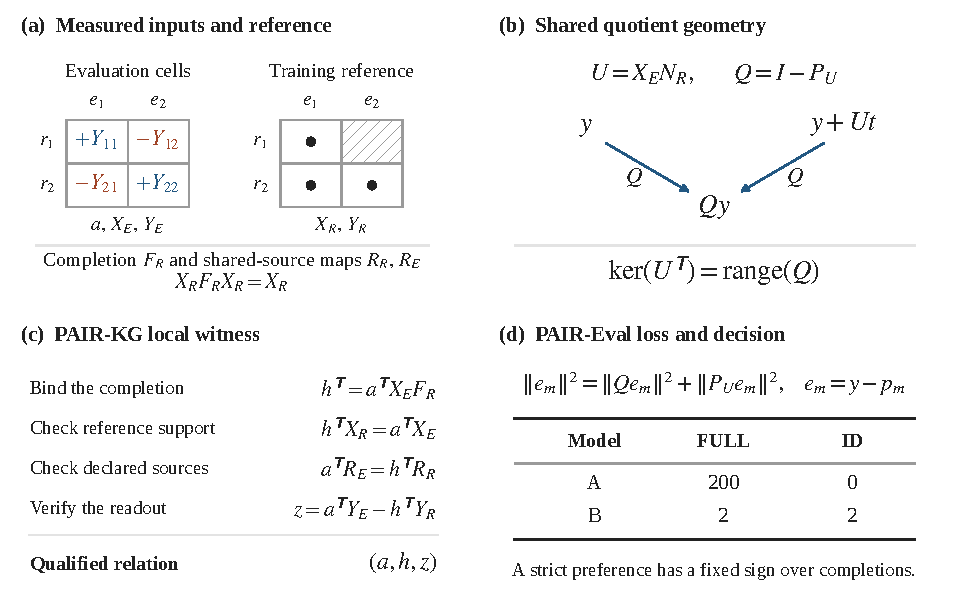
\includegraphics[width=\textwidth]{figures/figure_01.pdf}
\caption{\textbf{PAIR from measured inputs to verifiable relations and model evaluation.} \textbf{(a)} Observed query cells, an incomplete TRAIN reference, a registered completion $F_R$ and shared-source maps provide the inputs. Colored reference cells indicate measurements; gray cells are unmeasured. \textbf{(b)} The unresolved directions $U=X_EN_R$ define the quotient projector $Q=I-P_U$: common unresolved shifts leave admissible differences unchanged, and $\ker(U^\top)=\operatorname{range}(Q)$ links comparison coefficients to resolved response components. \textbf{(c)} PAIR-KG checks reference support, binds the completion and tests declared-source cancellation, retaining all signed endpoints and a local witness in each qualified relation. \textbf{(d)} PAIR-Eval separates fixed prediction errors into resolved and unresolved components and certifies strict preferences over a bounded completion set. The table is an exact algebraic illustration, not a benchmark result: for $y=(10,8)^\top$, $p_A=(0,-2)^\top$, $p_B=(9,9)^\top$ and within-pair centering $Q$, squared losses are $(200,2)$ under FULL and $(0,2)$ under ID. Each application uses its own reference. The schematic was prepared with OpenAI ChatGPT (GPT-6.1 through Codex; November 2026) assistance for deterministic vector-drawing code.}
\label{fig:overview}
\end{figure}


\section{The \method unified framework}\label{sec:framework}

\subsection{System architecture and four-component input binding}
\method organizes both relational compilation and model evaluation around complete comparative functionals and their reference geometry. Each execution binds four mathematical objects:
\begin{enumerate}[label=(\roman*)]
\item the query contrast coefficient vector $a \in \R^{n_E}$ and measured evaluation response vector $Y_E \in \R^{n_E}$;
\item the frozen training reference design and response pair $(X_R, Y_R) \in \R^{n_R \times p} \times \R^{n_R}$;
\item a pre-registered linear reference completion operator $F_R \in \R^{p \times n_R}$ belonging to the generalized-inverse class
\[
\mathfrak{F}(X_R) = \{F \in \R^{p \times n_R} : X_R F X_R = X_R\},
\]
which produces the reference parameter estimate $\widehat{\theta}_R = F_R Y_R$ (e.g., unweighted Moore--Penrose OLS $F_R = X_R^+$ or precision-weighted training WLS); and
\item optional declared shared-source incidence matrices $R_R \in \R^{n_R \times q}$ and $R_E \in \R^{n_E \times q}$ encoding how $q$ shared controls, capture batches, or technical offsets enter the reference and evaluation rows.
\end{enumerate}
The generalized-inverse condition $X_R F_R X_R = X_R$ ensures that the fitted reference predictor $X_R \widehat{\theta}_R = X_R F_R Y_R$ acts as the identity on $\col(X_R)$. From this common binding, \pairkg compiles verified quantitative relations while \paireval scores competing predictive models on the reference-resolved subspace.

\subsection{\pairkg: Completion-bound, source-qualified relational compilation}\label{subsec:kg}

\paragraph{Completion-bound readout}
When a candidate contrast $a \in \R^{n_E}$ satisfies the reference-estimability condition $a^\top U = 0$, Theorem~\ref{eq:duality} guarantees $a^\top X_E \in \row(X_R)$. Under the registered completion operator $F_R$, \pairkg computes the \emph{reference completion witness} $h \in \R^{n_R}$ and the \emph{reference-completed readout} $z_{F_R}(a) \in \R$:
\begin{equation}\label{eq:readout}
h^\top = a^\top X_E F_R, \qquad z_{F_R}(a) = a^\top Y_E - h^\top Y_R.
\end{equation}
Crucially, $z_{F_R}(a)$ is a property of the \emph{entire contrast tuple} $(a, X_R, Y_R, F_R)$, not an isolated atomic edge weight. Why must $F_R$ be explicitly bound if $a^\top U = 0$ already ensures parameter estimability? When the finite-sample reference vector $Y_R$ contains noise or interaction residuals outside $\col(X_R)$ and $a^\top X_E \neq 0$, the induced estimable reference functional agrees on $\col(X_R)$ across valid completions, while its action on out-of-column reference residuals can differ. Indeed, if $F_R$ is left unspecified across $\mathfrak{F}(X_R)$ and $Y_R \notin \col(X_R)$ with $a^\top X_E \neq 0$, the set of attainable readouts $\{a^\top Y_E - a^\top X_E F Y_R : F \in \mathfrak{F}(X_R)\}$ spans the entire real line $\R$ (Supplementary Section~S1.1.3, Proposition~1). Binding $F_R$ and $h$ eliminates this finite-sample completion ambiguity.

\paragraph{Declared-source qualification and local verification}
Suppose an unmeasured vector of shared control or batch offsets $u \in \R^q$ contributes additively to the reference and evaluation responses via $R_R u$ and $R_E u$. After reference completion under $F_R$, the net contribution of $u$ to the completed readout $z_{F_R}(a)$ is $(a^\top R_E - h^\top R_R)u = a^\top (R_E - X_E F_R R_R) u$. Defining the \emph{residual source operator}
\[
J = R_E - X_E F_R R_R \in \R^{n_E \times q},
\]
the \emph{jointly qualified contrast subspace} $\mathcal{L}$ that simultaneously annihilates training-unresolved reference parameters and declared shared sources is
\begin{equation}\label{eq:jointgate}
\begin{aligned}
\mathcal{L} &= \ker([U\ \ J]^\top) = \ker(U^\top) \cap \ker(J^\top),\\
a \in \mathcal{L} &\iff a^\top U = 0 \ \ \text{and}\ \ a^\top J = 0.
\end{aligned}
\end{equation}
Equation~\eqref{eq:jointgate} upgrades passive provenance lineage into an active algebraic invariance gate: rather than merely logging that a query touched control group $u$, $a^\top J = 0$ certifies that $u$ cancels out of the completed numerical value $z_{F_R}(a)$.

\begin{proposition}[Reference and declared-source cancellation, local witness, and aggregation closure]\label{prop:soundness}
Suppose the reference and evaluation responses follow the structural decomposition
\[
Y_R = X_R \theta + \Gamma_R + R_R u + \varepsilon_R, \qquad Y_E = X_E \theta + \Gamma_E + R_E u + \varepsilon_E,
\]
with registered completion operator $F_R \in \mathfrak{F}(X_R)$ satisfying $X_R F_R X_R = X_R$ and witness $h^\top = a^\top X_E F_R$. Then:
\begin{enumerate}[label=(\roman*)]
\item \textbf{Exact nuisance cancellation:} If $a \in \mathcal{L}$, then for all $\theta \in \R^p$ and $u \in \R^q$, the completed readout eliminates both the reference parameter $\theta$ and the declared source vector $u$:
\begin{equation}\label{eq:soundness}
z_{F_R}(a) = a^\top \Gamma_E - h^\top \Gamma_R + a^\top \varepsilon_E - h^\top \varepsilon_R.
\end{equation}
\item \textbf{Four-equation local verification witness:} A candidate record $(a, h, z)$ is completion-bound, reference-estimable, declared-source-safe, and numerically consistent with $(X_R, Y_R, X_E, Y_E, F_R, R_R, R_E)$ if and only if it satisfies the four local linear identities
\begin{equation}\label{eq:fourwitness}
\begin{aligned}
h^\top &= a^\top X_E F_R, & h^\top X_R &= a^\top X_E,\\
a^\top R_E &= h^\top R_R, & z &= a^\top Y_E - h^\top Y_R.
\end{aligned}
\end{equation}
\item \textbf{Subspace and witness closure:} For any collection of qualified contrasts $\{a_k\}_{k=1}^m \subset \mathcal{L}$ compiled under the same ordered support, reference design, completion operator $F_R$, and source ledger, any linear combination $a_{\mathrm{agg}} = \sum_{k=1}^m \gamma_k a_k$ ($\gamma_k \in \R$) satisfies $a_{\mathrm{agg}} \in \mathcal{L}$ with composite witness $h_{\mathrm{agg}} = \sum_{k=1}^m \gamma_k h_k$ and readout $z_{F_R}(a_{\mathrm{agg}}) = \sum_{k=1}^m \gamma_k z_{F_R}(a_k)$.
\end{enumerate}
\end{proposition}
\begin{proof}
By Theorem~\ref{eq:duality}, $a^\top U = 0$ holds if and only if $a^\top X_E = c^\top X_R$ for some $c \in \R^{n_R}$. Using $X_R F_R X_R = X_R$, we obtain
\[
h^\top X_R = a^\top X_E F_R X_R = c^\top X_R F_R X_R = c^\top X_R = a^\top X_E.
\]
Conversely, $h^\top X_R = a^\top X_E$ implies $a^\top X_E \in \row(X_R)$, so $a^\top U = 0$. Moreover, $a^\top J = a^\top(R_E - X_E F_R R_R) = a^\top R_E - h^\top R_R$, which vanishes if and only if $a^\top R_E = h^\top R_R$. Substituting the structural decompositions of $Y_R$ and $Y_E$ into $z_{F_R}(a) = a^\top Y_E - h^\top Y_R$ yields
\[
\begin{aligned}
z_{F_R}(a) ={}& (a^\top X_E - h^\top X_R)\theta + (a^\top R_E - h^\top R_R)u\\
&+ a^\top \Gamma_E - h^\top \Gamma_R + a^\top \varepsilon_E - h^\top \varepsilon_R.
\end{aligned}
\]
When $a \in \mathcal{L}$, the first two terms vanish identically, proving (i) and (ii). Part (iii) follows immediately from the linearity of matrix multiplication and the subspace structure of $\mathcal{L} = \ker([U\ J]^\top)$.
\end{proof}

Proposition~\ref{prop:soundness} also implies a clean structural monotonicity property whenever a coarse source ledger is refined into finer technical or control strata (detailed in Supplementary Section~S13.1):

\begin{corollary}[Source-ledger refinement monotonicity and bounded sensitivity]\label{cor:refinement}
Under a fixed ordering and completion operator $F_R$, suppose a coarse source ledger $R^{\mathrm{coarse}} = (R_R^{\mathrm{coarse}}, R_E^{\mathrm{coarse}})$ is a linear aggregation $R_R^{\mathrm{coarse}} = R_R^{\mathrm{fine}} C$ and $R_E^{\mathrm{coarse}} = R_E^{\mathrm{fine}} C$ of a finer source ledger $R^{\mathrm{fine}}$ for some aggregation matrix $C$. Then the residual source operators satisfy $J(R^{\mathrm{coarse}}) = J(R^{\mathrm{fine}})C$, and the jointly qualified subspaces obey the nested inclusion
\[
\mathcal{L}(R^{\mathrm{fine}}) \subseteq \mathcal{L}(R^{\mathrm{coarse}}).
\]
Furthermore, if a contrast is evaluated under fine-ledger source perturbations bounded by $\|\delta u\|_2 \le \rho$, its worst-case source-induced readout bias is given exactly by the dual norm radius $\sup_{\|\delta u\|_2 \le \rho} |a^\top J(R^{\mathrm{fine}}) \delta u| = \rho \|a^\top J(R^{\mathrm{fine}})\|_2$.
\end{corollary}
\begin{proof}
By linearity, $J(R^{\mathrm{coarse}}) = R_E^{\mathrm{fine}}C - X_E F_R R_R^{\mathrm{fine}}C = J(R^{\mathrm{fine}})C$. Thus $a^\top J(R^{\mathrm{fine}}) = 0$ implies $a^\top J(R^{\mathrm{coarse}}) = 0$, yielding $\mathcal{L}(R^{\mathrm{fine}}) \subseteq \mathcal{L}(R^{\mathrm{coarse}})$. The exact sensitivity radius follows from the self-duality of the Euclidean norm via Cauchy--Schwarz.
\end{proof}

\begin{table}[t]
\centering\small\setstretch{1.05}
\caption{Four-stage compilation protocol and three-way epistemic terminal states in \pairkg.}
\label{tab:procedure}
\begin{tabularx}{\textwidth}{@{}L{0.25\textwidth}X@{}}
\toprule
Compilation Stage & Verification Operation and Terminal Status Assignment \\\midrule
1. Input \& provenance binding & Bind ordered query support, contrast coefficients $a$, reference version $(X_R, Y_R)$, completion operator $F_R$, source matrices $(R_R, R_E)$, and numerical tolerances. Legacy readouts with unbound source ledgers are capped at the boundary state \texttt{MEASUREMENT\_ONLY}. \\
2. Reference estimability gate & Construct $U = X_E N_R$ and verify $a^\top U = 0$ (equivalently $h^\top X_R = a^\top X_E$ across SVD and pivoted RRQR). Queries failing this gate are refused as \texttt{NOT\_IDENTIFIABLE}. \\
3. Declared-source safety gate & Compute $h^\top = a^\top X_E F_R$ under the identical operator $F_R$ and verify $a^\top R_E - h^\top R_R = 0$. Queries failing source cancellation are refused as \texttt{SOURCE\_UNSAFE}. \\
4. Readout \& witness emission & Evaluate $z_{F_R}(a) = a^\top Y_E - h^\top Y_R$ and audit all four local identities in Eq.~\eqref{eq:fourwitness}. Solver disagreements trigger \texttt{NUMERICALLY\_UNRESOLVED}; passing records are emitted as \texttt{ATOMIC\_ASSERTABLE} or \texttt{COMPARATIVE\_ASSERTABLE} with $(a, h, z_{F_R}(a))$. \\\bottomrule
\end{tabularx}
\end{table}

Table~\ref{tab:procedure} summarizes how \pairkg operationalizes Proposition~\ref{prop:soundness} as a four-stage compilation pipeline that partitions candidate requests into three epistemic strata: source-certified assertions (\texttt{ATOMIC\_ASSERTABLE}, \texttt{COMPARATIVE\_ASSERTABLE}), boundary measurement records (\texttt{MEASUREMENT\_ONLY}), and formal refusals (\texttt{NOT\_IDENTIFIABLE}, \texttt{SOURCE\_UNSAFE}, \texttt{NUMERICALLY\_UNRESOLVED}).

\subsection{\paireval: Quotient-space targets and model-order invariance}\label{subsec:eval}
We now turn to the dual branch of \method: evaluating competing predictive models $p_1, \dots, p_M \in \R^{n_E}$ against the held-out response vector $y = Y_E \in \R^{n_E}$. Because $Q = I_{n_E} - P_U$ and $P_U$ are complementary orthogonal projectors ($\operatorname{range}(Q) \perp \col(U)$), the ambient squared prediction error $L_m^{\mathrm{FULL}}$ decomposes orthogonally for every predictor $p_m$:
\begin{equation}\label{eq:scoredecomp}
\underbrace{\|y - p_m\|_2^2}_{L_m^{\mathrm{FULL}}} = \underbrace{\|Q(y - p_m)\|_2^2}_{L_m^{\mathrm{ID}}} + \underbrace{\|(I_{n_E} - Q)(y - p_m)\|_2^2}_{\text{unresolved-subspace error}}.
\end{equation}
Thus, ambient scoring (\texttt{FULL}) and reference-resolved quotient scoring (\texttt{ID}) evaluate two mathematically distinct target definitions on the exact same emitted predictions: $L_m^{\mathrm{ID}}$ measures accuracy strictly on the reference-identifiable contrast space $\operatorname{range}(Q)$, whereas $L_m^{\mathrm{FULL}}$ adds the squared residual on the training-unresolved subspace $\col(U)$. (When a benchmark additionally restricts evaluation to a declared source-safe subspace $\mathcal{L} = \ker([U\ J]^\top)$, $Q$ is replaced by the joint orthogonal projector $Q_{\mathcal{C}} = I - P_{[U\ J]}$ derived in Supplementary Section~S1.4.2.)

To formalize how unresolved reference directions affect pairwise model ranking, let $W \succeq 0$ be a symmetric positive-semidefinite scoring weight matrix shared by two competing predictors $p_A, p_B \in \R^{n_E}$. Consider a \emph{truth-only reference-completion shift} $y(t) = y + Ut$ ($t \in \R^k$), which shifts the baseline-adjusted evaluation target along the training-unresolved subspace $\col(U)$ while holding the emitted model predictions $p_A, p_B$ fixed. Expanding the weighted squared-loss difference $\Delta_{A,B}(t) = \|y(t) - p_A\|_W^2 - \|y(t) - p_B\|_W^2$ yields the exact affine functional
\begin{equation}\label{eq:decisionaffine}
\Delta_{A,B}(t) = \Delta_{A,B}(0) + 2 t^\top U^\top W (p_B - p_A),
\end{equation}
because the quadratic target term $t^\top U^\top W U t$ is identical for both models and cancels in the pairwise difference.

\begin{proposition}[Model-order invariance under truth-only completion shifts]\label{prop:order}
For fixed predictions $p_A, p_B \in \R^{n_E}$ and shared weight matrix $W \succeq 0$ under truth-only reference-completion shifts $y(t) = y + Ut$ across $t \in \R^k$:
\begin{enumerate}[label=(\roman*)]
\item The pairwise loss difference $\Delta_{A,B}(t)$ is invariant for all $t \in \R^k$ if and only if $U^\top W (p_B - p_A) = 0$. In particular, choosing the quotient scoring operator $W = Q$ guarantees $U^\top Q = 0$, rendering the reference-resolved loss difference $\Delta_{A,B}^{\mathrm{ID}}(t) = L_A^{\mathrm{ID}}(t) - L_B^{\mathrm{ID}}(t)$ strictly invariant for all prediction pairs $(p_A, p_B)$.
\item Under ambient unweighted scoring ($W = I_{n_E}$), if the prediction difference has a nonzero projection onto the unresolved subspace ($U^\top(p_B - p_A) \neq 0$), then $\{\Delta_{A,B}^{\mathrm{FULL}}(t) : t \in \R^k\} = \R$, so both strict model orderings ($A \succ B$ and $B \succ A$) are attainable across training-compatible reference completions.
\end{enumerate}
\end{proposition}
\begin{proof}
By Eq.~\eqref{eq:decisionaffine}, $\Delta_{A,B}(t)$ is an affine function of $t \in \R^k$ with gradient $\nabla_t \Delta_{A,B}(t) = 2 U^\top W (p_B - p_A)$. An affine functional on $\R^k$ is constant if and only if its gradient vanishes, and surjects onto $\R$ whenever its gradient is nonzero. Setting $W = Q$ gives $U^\top Q = (QU)^\top = 0$, so $\nabla_t \Delta_{A,B}^{\mathrm{ID}}(t) = 0$ identically for all $p_A, p_B$. Setting $W = I_{n_E}$ with $s = U^\top(p_B - p_A) \neq 0$ allows $t = \alpha s$ ($\alpha \in \R$) to drive $\Delta_{A,B}^{\mathrm{FULL}}(\alpha s) = \Delta_{A,B}^{\mathrm{FULL}}(0) + 2\alpha \|s\|_2^2$ to any real value.
\end{proof}

\begin{remark}[Truth-only shifts, joint translations, and bounded three-way decision regimes]
Proposition~\ref{prop:order} highlights a crucial distinction between three operations on held-out evaluations: (i) applying a \emph{joint translation} $(y, p_1, \dots, p_M) \mapsto (y + Ut, p_1 + Ut, \dots, p_M + Ut)$ to both the ground truth and all predictions simultaneously, which leaves every residual $y - p_m$ and all common-support SSE rankings invariant (Supplementary Section~S1.6); (ii) applying a \emph{truth-only completion shift} $y \mapsto y + Ut$ with fixed emitted predictions $p_m$, which induces the affine drift in Eq.~\eqref{eq:decisionaffine}; and (iii) applying the \emph{quotient projector} $Q$, which strips the unresolved residual $\|(I-Q)(y-p_m)\|_2^2$ even at $t=0$. When domain knowledge restricts $t$ to a compact polytope $\mathcal{T} = \{t \in \R^k : C t \le d\}$ rather than $\R^k$, linear programming over Eq.~\eqref{eq:decisionaffine} partitions model comparisons into a three-way decision structure~\cite{li2026incomplete,zhang2026adaptive}: strictly invariant preference for $A$ ($\max_{t \in \mathcal{T}} \Delta_{A,B}(t) < 0$), strictly invariant preference for $B$ ($\min_{t \in \mathcal{T}} \Delta_{A,B}(t) > 0$), or a boundary regime without a certified strict preference, where the interval $[\min_{t \in \mathcal{T}}\Delta_{A,B}(t), \max_{t \in \mathcal{T}}\Delta_{A,B}(t)]$ contains zero. This boundary distinguishes a fixed tie from a one-sided tie boundary or genuinely variable strict orders (Supplementary Sections~S5 and S14).
\end{remark}

\subsection{Universal completion invariance of balanced four-cell contrasts}\label{subsec:independence}
For a general reference-estimable query satisfying $w^\top = a^\top X_E \in \row(X_R) \setminus \{0\}$, the witness $h^\top = w^\top F_R$ is nonzero, so the completed readout $z_{F_R}(a)$ and residual source exposure $a^\top J$ depend on the specific choice of generalized inverse $F_R \in \mathfrak{F}(X_R)$. However, an important subclass of comparative queries achieves \emph{universal invariance across the entire generalized-inverse family} $\mathfrak{F}(X_R)$ (proved in full generality in Supplementary Section~S16, Proposition~8):

\begin{proposition}[Universal completion invariance across $\mathfrak{F}(X_R)$]\label{prop:fourcell}
Let $a \in \R^{n_E}$ be a reference-estimable query ($w^\top = a^\top X_E \in \row(X_R)$). The completed readout $z_F(a) = a^\top Y_E - w^\top F Y_R$ and declared-source residual $s_F(a) = a^\top R_E - w^\top F R_R$ are invariant across all generalized inverses $F \in \mathfrak{F}(X_R)$ if and only if either $w = 0$ or every column of $[Y_R\ \ R_R]$ lies in $\col(X_R)$. In particular, for any balanced four-cell interaction contrast $a = (+1, -1, -1, +1)^\top$ on a pure two-way additive reference design $X_E$, the query coefficients annihilate the evaluation design directly ($w^\top = a^\top X_E = 0$), yielding
\[
h^\top = a^\top X_E F = 0, \qquad z_F(a) = a^\top Y_E, \qquad s_F(a)=a^\top R_E,\qquad \text{source contribution}=s_F(a)u
\]
identically for every $F \in \mathfrak{F}(X_R)$.
\end{proposition}
\begin{proof}
If $w = 0$, then $h^\top = w^\top F = 0$ for every $F \in \mathfrak{F}(X_R)$, so $z_F(a) = a^\top Y_E$ and $s_F(a) = a^\top R_E$ are independent of $F$. If $V = [Y_R\ R_R] = X_R B$ and $w^\top = c^\top X_R$, then $w^\top F V = c^\top X_R F X_R B = c^\top X_R B$ for all $F \in \mathfrak{F}(X_R)$. Conversely, if $w \neq 0$ and some column $v_0$ of $V$ lies outside $\col(X_R)$, there exist $q \in \ker(X_R^\top)$ with $q^\top v_0 \neq 0$ and $u \in \R^p$ with $w^\top u \neq 0$; perturbing $F \mapsto F + u q^\top \in \mathfrak{F}(X_R)$ shifts $w^\top F v_0$ by $(w^\top u)(q^\top v_0) \neq 0$. For a balanced four-cell contrast on a pure two-way additive design, the alternating weights $(+1,-1,-1,+1)$ sum to zero within each regulator and event margin, giving $a^\top X_E = 0$.
\end{proof}

Proposition~\ref{prop:fourcell} explains why balanced four-cell interaction queries occupy a privileged algebraic position: when all four cells are measured on a pure additive reference design and share an equal-weight control mapping ($a^\top R_E = 0$), both reference completion and shared-source cancellation hold universally without depending on the reference response $Y_R$. At the same time, four-cell syntax alone cannot impute an unmeasured evaluation cell or automatically cancel unequal batch weights or nonlinear within-batch $z$-score rescaling, which is why \pairkg always verifies the actual support and declared source matrices.

\subsection{Algorithmic realization and computational complexity}\label{subsec:complexity}
The implementation separates one-time reference geometry, numerical completion, local witness verification and fixed-prediction scoring. The following are arithmetic bounds for the specified representations, not measured runtime comparisons.
\begin{enumerate}
\item \textbf{Reference geometry.} Write $r=\rank(X_R)$, $k=p-r$ and $r_U=\rank(U)$. A full right null-space basis can be obtained from a dense SVD with a conservative $O(n_Rp^2)$ bound; forming $U=X_EN_R$ costs $O(n_Epk)$. Standard dense rank-revealing factorization of the $n_E\times k$ matrix $U$ costs $O(n_Ek\min\{n_E,k\})$, giving
\[
\mathcal T_{\mathrm{geometry}}
=O\!\left(n_Rp^2+n_Epk+n_Ek\min\{n_E,k\}\right).
\]
The ordinary tall-matrix case uses $n_R\ge p$; full right-basis formation is included in the conservative bound for a wider reference. Materializing $X_R,X_E,N_R,U$ and an orthonormal basis $B_U\in\R^{n_E\times r_U}$ requires $O(n_Rp+n_Ep+pk+n_Ek+n_Er_U)$ storage. Sparse or graph-specific representations can reduce these costs. For a pure two-way incidence design, preprocessing connected components and checking endpoint connectivity take linear graph time; this special-case eligibility check does not itself compute a numerical completion or source witness.
\item \textbf{Compilation and complete local verification.} Precomputing $F_RY_R$ and $F_RR_R$ can reuse the registered completion representation. Query work then depends on the nonzeros in the rows touched by $a$, the retained rank and source width. Emitting the completion-bound witness additionally requires $h=F_R^\top X_E^\top a$. Let $\mathcal T_{F_R^\top}$ denote the cost of applying the \emph{registered} transposed completion to one vector. A complete check of all four identities in Eq.~\eqref{eq:fourwitness} has the bound
\begin{equation}\label{eq:verifycost}
\begin{aligned}
\mathcal T_{\mathrm{verify}}=O\big(&\nnz(X_R)+\nnz(X_E)+\nnz(R_R)+\nnz(R_E)\\
&+\mathcal T_{F_R^\top}+n_R+n_E+p+q\big).
\end{aligned}
\end{equation}
If $F_R$ is explicitly stored sparsely, $\mathcal T_{F_R^\top}=O(\nnz(F_R))$; an explicit dense $F_R$ instead costs $O(pn_R)$. A factorized representation carries its own application cost. The additional vector workspace is $O(n_R+n_E+p+q)$, beyond stored operators. Thus verification uses matrix--vector operations and can avoid a new reference factorization when the registered completion representation is available; its cost cannot omit that completion-binding operation.
\item \textbf{Low-rank quotient scoring.} Once $B_U$ has been constructed, the action $Qv=v-B_U(B_U^\top v)$ costs $O(n_E(r_U+1))$ without storing a dense $n_E\times n_E$ projector. Evaluating the projected residuals and scalar scores for $M$ models costs $O(Mn_E(r_U+1))$, including the identity case $r_U=0$. The stored basis uses $O(n_Er_U)$ memory and one-vector workspace uses $O(n_E+r_U)$. Under the ordinary connected LDO/LCO geometry, within-held-out-group centering gives $O(Mn_E)$ scoring. Explicit enumeration of every model-pair direction is a separate $O(M^2)$ diagnostic per fold and metric.
\end{enumerate}

\section{Experimental design and evaluation protocols}\label{sec:design}

We evaluate \method across four large-scale molecular perturbation resources and three pharmacogenomic drug-response benchmarks, organized around three primary research questions (Table~\ref{tab:resources}):
\begin{itemize}
\item \textbf{RQ1 (Compound subspace retention and cross-replicate coherence):} How much identifiable comparative information in incomplete perturbation screens exists exclusively as multi-cell compound contrasts beyond atomic coordinates, and do these source-qualified subspaces retain cross-replicate common-response structure?
\item \textbf{RQ2 (Reference support verification, completion replay, and shared-source cancellation):} Can syntactic query-type templates substitute for exact reference-support verification ($a^\top U = 0$), how sensitive are completed readouts to reference-version shifts, and does \pairkg certify exact shared-control cancellation on native additive measurement scales?
\item \textbf{RQ3 (Quotient target specification and cross-fold preference persistence):} How does replacing ambient evaluation (\texttt{FULL}, $T=I$) with reference-resolved quotient evaluation (\texttt{ID}, $T=Q$) alter fixed-prediction model rankings, and which pairwise preference reversals persist across cross-validation folds, external cohorts, and symmetric hyperparameter retraining?
\end{itemize}

\begin{table}[t]
\centering\small\setstretch{1.05}
\caption{Summary of research questions, empirical resources, observation supports, and primary evaluation protocols.}
\label{tab:resources}
\begin{tabularx}{\textwidth}{@{}L{0.12\textwidth}L{0.42\textwidth}X@{}}
\toprule
Question & Empirical Resources and Support Geometry & Primary Evaluation Protocol \\\midrule
RQ1 & K562 APA~\cite{kowalski2024cpa} ($150$ inner mask exposures; $5$ strict new-event replicate folds); ENCODE RBP splicing~\cite{vannostrand2020rbp} ($20$ masks; $506{,}626$ events); HEK293T PAS-seq~\cite{jagannatha2026rbp} ($5$ strict new-event folds; $30{,}198$ pairs) & Compound-only subspace dimension in $\ker(U^\top)$ orthogonal to individually estimable coordinate directions; basis-invariant replicate covariance $\widehat{S}$ (Eq.~\eqref{eq:replicate}); 10-mask comparison-supervision diagnostic. \\
RQ2 & K562 APA ($50$ outer supports, $10{,}182{,}954$ candidate requests; fold-0 $3{,}125$ historical queries; $150$ inner reference versions); Replogle K562 Perturb-seq~\cite{replogle2022perturbseq} ($310{,}385$ cells, $8{,}563$ genes, $48$ GEMs, $97$ NTC guides, $100{,}000$ Q4 designs, $128$ two-GEM pools) & Null-space / bipartite connectivity vs. syntactic query-type shortcuts; conditional OLS numerical replay ($2.3 \times 10^{-14}$); V3 shared-control cancellation ($\delta_{\mathrm{source}}=0$) and within-group $z$-score distortion analysis. \\
RQ3 & CTRPv2~\cite{rees2016ctrp,bernett2026dreval} ($7$ LDO predictors, $10$ folds, registered model-specific supports); GDSC2 \& GDSC1~\cite{iorio2016gdsc} ($6$-model common support + fingerprint-only expansion); $560$-job symmetric-HPO retraining control & DrEval baseline-normalized $\mathrm{n}R^2$ and $\mathrm{n}r$ under $T \in \{I, Q\}$; fold-wise pairwise reversal fraction; prespecified $\ge 7/10$-fold directional persistence and two-part GDSC2 confirmation gate. \\\bottomrule
\end{tabularx}
\end{table}

\subsection{Molecular perturbation resources and structural summaries (RQ1--RQ2)}
The molecular perturbation experiments draw on four large-scale transcriptomic resources~\cite{kowalski2024cpa,vannostrand2020rbp,jagannatha2026rbp,replogle2022perturbseq} (preprocessing definitions, available data hashes, and reproduction scopes are documented in Supplementary Sections~S2 and S6). For each reference--evaluation mask, the \emph{compound-only dimension} is defined as the algebraic dimension of the reference-estimable contrast space $\ker(U^\top)$ remaining after projecting out all individually estimable atomic coordinate directions ($e_j \in \ker(U^\top)$). Because mask exposures reuse the underlying assay matrix across splits, cumulative dimension counts across masks quantify structural design capacity across repeated split exposures rather than independent biological sample size.

To test whether a source-qualified contrast subspace of dimension $d > 0$ captures reproducible biological signal across experimental replicates rather than random noise, let $B \in \R^{d \times n_E}$ be any full-row-rank basis matrix for the qualified contrast space, and let $z_1, z_2 \in \R^d$ denote the completed contrast vectors computed on replicate channels 1 and 2. We evaluate the basis-invariant \emph{replicate-common covariance summary}:
\begin{equation}\label{eq:replicate}
\widehat{S} = \frac{z_1^\top (B B^\top)^{-1} z_2}{d}.
\end{equation}
For any invertible basis transformation $B \mapsto A B$ ($A \in \mathrm{GL}_d(\R)$), the replicate vectors transform as $z_i \mapsto A z_i$ and $(A B B^\top A^\top)^{-1} = A^{-\top}(B B^\top)^{-1}A^{-1}$, leaving $\widehat{S}$ strictly invariant. Thus, $\widehat{S}$ measures the mean whitened cross-replicate covariance per qualified degree of freedom on each assay's native response scale.

\subsection{Pharmacogenomic prediction panels and persistence protocol (RQ3)}
Our primary drug-response evaluation examines the seven fixed CTRPv2 leave-drug-out (LDO) predictors archived under the DrEval~\cite{bernett2026dreval} benchmarking suite across ten outer cross-validation folds: \texttt{DIPK}, \texttt{ElasticNet}, \texttt{GradientBoosting}, \texttt{MultiOmicsNeuralNetwork}, \texttt{MultiOmicsRandomForest}, \texttt{RandomForest}, and \texttt{SimpleNeuralNetwork}. Following DrEval v1.4.1, let $b$ denote the fold-specific \texttt{NaiveMeanEffects} additive baseline evaluated on the aligned test rows. For target operator $T = I$ (\texttt{FULL}) or $T = Q$ (\texttt{ID}), we compute baseline-centered responses and predictions together with baseline-normalized $R^2$ ($\mathrm{n}R_m^2$) and baseline-normalized Pearson correlation ($\mathrm{n}r_m$):
\begin{equation}\label{eq:normalized}
\begin{aligned}
y_T &= T(y - b), \qquad p_{m,T} = T(p_m - b),\\
\mathrm{n}R_m^2 &= R^2(y_T, p_{m,T}), \qquad \mathrm{n}r_m = \operatorname{corr}(y_T, p_{m,T}).
\end{aligned}
\end{equation}
In CTRPv2, each archived predictor is evaluated on its registered post-merge observation support using its matched baseline $b$ and design-derived projector $Q$; for standard connected LDO bipartite topologies, $Q$ coincides algebraically with within-held-out-drug centering, while disconnected GDSC supports use the exact pseudoinverse projector in Eq.~\eqref{eq:sharedspace} (Supplementary Section~S4.7).

Within each fold and metric, the \emph{pairwise reversal fraction} is defined as the proportion of evaluated model pairs $(A,B)$ whose strict score preference reverses sign between \texttt{FULL} and \texttt{ID} (exceeding the numerical tie tolerance; tie-to-strict changes are not counted as reversals). A directed pair--metric reversal is classified as \emph{persistent} when the exact same \texttt{FULL}-to-\texttt{ID} sign reversal occurs in at least $7$ of the $10$ outer folds. In our pre-registered GDSC2 confirmation protocol (evaluated on the six-model common support excluding \texttt{DIPK} due to missing drug molecular graphs, with \texttt{DIPK} analyzed in a companion check), study-level confirmation requires both a median fold-level reversal fraction $\ge 0.10$ and at least one persistent ($\ge 7/10$ folds) directed pair--metric reversal. To separate scoring-target effects on fixed predictions from retraining variability, we additionally execute a 560-job symmetric hyperparameter optimization (HPO) retraining control (Supplementary Section~S4.8).

\section{Empirical results}\label{sec:results}

\subsection{RQ1: Compound comparisons retain substantial information and replicate coherence beyond atomic effects}\label{subsec:result-space}

Restricting a knowledge base or benchmark to individually estimable atomic coordinates discards a large fraction of the comparative information identified by incomplete reference designs. Across $150$ frozen K562 APA mask exposures, $9{,}945$ baseline-adjusted coordinate exposures fail individual atomic estimability ($e_j^\top U \neq 0$), yet the training reference designs uniquely identify \textbf{$2{,}635$ compound-only dimensions} ($\ker(U^\top)$ directions orthogonal to the individually estimable coordinate directions), representing \textbf{$26.50\%$} of the atomically unsupported exposures (Fig.~\ref{fig:internal}a and Table~\ref{tab:rq12_summary}). A consistent geometric phenomenon emerges at genome scale across $20$ ENCODE RBP splicing masks: out of $973{,}298$ atomically unsupported coordinate exposures, the reference designs retain \textbf{$56{,}395$ compound-only dimensions ($5.79\%$)} that exist exclusively as multi-cell linear contrasts.

\begin{figure}[t]
\centering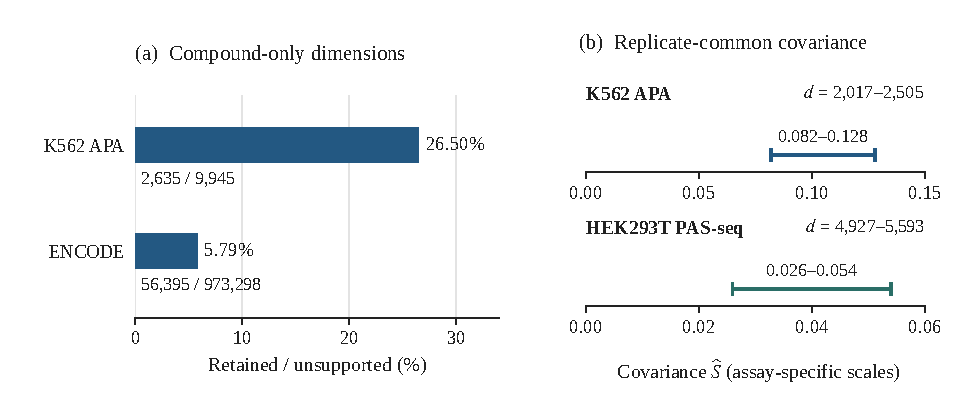
\includegraphics[width=\textwidth]{figures/figure_02.pdf}
\caption{\textbf{Compound subspace retention and cross-replicate coherence under incomplete reference designs (RQ1).} \textbf{(a)} Decomposition of atomically unsupported coordinate exposures versus dimensions retained exclusively through compound linear contrasts ($\ker(U^\top)$) across 150 K562 APA mask exposures ($2{,}635 / 9{,}945 = 26.50\%$) and 20 ENCODE splicing masks ($56{,}395 / 973{,}298 = 5.79\%$). \textbf{(b)} Source-qualified subspace dimensions $d$ and basis-invariant replicate-common covariance $\widehat{S}$ (Eq.~\eqref{eq:replicate}) across five frozen K562 folds ($d \in [2{,}017, 2{,}505]$, $\widehat{S} \in [0.082, 0.128]$) and five strict new-event HEK293T PAS-seq folds ($d \in [4{,}927, 5{,}593]$, $\widehat{S} \in [0.026, 0.054]$).}
\label{fig:internal}
\end{figure}

The retained compound subspaces also exhibit positive shared response structure across the stored replicate channels. As shown in Fig.~\ref{fig:internal}b, the basis-invariant replicate-common statistic $\widehat{S}$ (Eq.~\eqref{eq:replicate}) is strictly positive across all five frozen K562 APA replicate folds, ranging from $\widehat{S} = 0.082$ to $0.128$ over source-qualified subspaces of dimension $d \in [2{,}017, 2{,}505]$. We observe positive cross-replicate alignment in the independent HEK293T tethered PAS-seq screen across five strict new-event folds, where $\widehat{S}$ ranges from $0.026$ to $0.054$ over source-qualified dimensions $d \in [4{,}927, 5{,}593]$.

Companion replay and supervision diagnostics in Supplementary Sections~S3 and S8 further contextualize how predictive learners utilize this subspace. The historical K562 low-dimensional B2 baseline has mean squared loss $0.1129436318$, compared with $0.1905898683$ for zero D3, a $40.740\%$ reduction under its original 50-mask target definition. Meanwhile, in our 10-mask post-hoc comparison-supervision diagnostic (Supplementary Section~S8, Table~S7), training a rank-four model via four-term contrast supervision versus raw-response supervision yields nearly identical calibrated evaluation loss ($0.8364$ vs. $0.8354$, difference $+0.0010$, against $1.0000$ for additive predictions and $0.7296$ for a held-out replicate R1 positive control), consistent with the exact GLS row-space equivalence $(Be)^\top(BB^\top)^{-1}(Be) = e^\top P_{\row(B)}e$. Together, these findings establish that compound contrasts preserve substantial, replicate-coherent experimental information that atomic catalogues discard.

\begin{table}[t]
\centering\small\setstretch{1.05}
\caption{Summary of empirical results for subspace retention (RQ1) and verifiable relational compilation (RQ2).}
\label{tab:rq12_summary}
\begin{tabularx}{\textwidth}{@{}L{0.18\textwidth}L{0.22\textwidth}XX@{}}
\toprule
Study / Benchmark & Evaluated Quantity & Observed Empirical Result & Methodological Implication \\ \midrule
K562 APA (150 masks) & Compound-only vs. unsupported atomic dims & $2{,}635 / 9{,}945$ ($26.50\%$) retained in $\ker(U^\top)$ & The compound-only dimensional retention ratio is $26.50\%$. \\
ENCODE RBP (20 masks) & Compound-only vs. unsupported atomic dims & $56{,}395 / 973{,}298$ ($5.79\%$) retained in $\ker(U^\top)$ & Tens of thousands of splicing contrasts survive exclusively as multi-cell functionals. \\
K562 \& HEK293T folds & Replicate-common coherence $\widehat{S}$ (dim $d$) & K562: $\widehat{S}\in [0.082, 0.128]$ ($d\in [2{,}017, 2{,}505]$); HEK293T: $\widehat{S}\in [0.026, 0.054]$ ($d\in [4{,}927, 5{,}593]$) & Source-qualified contrast spaces capture reproducible cross-replicate signal. \\
K562 50 outer supports & Syntactic query-type shortcut vs. exact $U^\top a = 0$ & Shortcut matches exact qualification on only $24.10\%$ of $10{,}182{,}954$ requests & Syntactic coefficient templates cannot replace training-support estimability checks. \\
K562 fold-0 replay & $3{,}125$ candidate queries ($349$ retained comparative terminals) & $100\%$ status \& readout replay to max discrepancy $2.3 \times 10^{-14}$ ($2{,}776$ nonidentifiable terminals) & The recovered reference conditionally reproduces the archived labels and retained readouts. \\
K562 150 inner splits & Reference-version sensitivity ($657$ repeated keys) & $657 / 657$ ($100\%$) shift by $>10^{-8}$; $14$ (R1) \& $17$ (R2) keys flip sign across splits & Relational records must bind the reference version and witness $h$ to remain well-defined. \\
Replogle Perturb-seq & $100{,}000$ four-cell (Q4) designs across $48$ GEMs & $100{,}000$ query designs satisfy $\delta_{\mathrm{source}}=0$; native-scale amplitudes require their declared measurement operator & Alternating contrasts cancel equal-weight GEM controls exactly on the native additive scale. \\ \bottomrule
\end{tabularx}
\end{table}

\subsection{RQ2: Reference support verification, completion replay, and shared-source cancellation}\label{subsec:result-kg}

Our second set of experiments examines syntactic query templates, completion binding, and \pairkg's explicit reference and source gates (Table~\ref{tab:rq12_summary}). First, across $50$ outer K562 reference supports generating $10{,}182{,}954$ candidate query exposures, a syntactic query-type shortcut that inspects only coefficient patterns without testing the actual training design $X_R$ agrees with exact reference-specific qualification on just \textbf{$24.10\%$} of requests (Supplementary Section~S10.2). In contrast, \pairkg's null-space test $a^\top U = 0$ agrees identically ($100\%$) with classical row-space inclusion and bipartite graph-connectivity checks on matched supports. Thus, a candidate contrast becomes a well-defined quantitative statement only after its specific training reference support is verified.

Second, for accepted queries, the numerical readout must be reproducible and explicitly tied to its reference completion. On the recovered K562 fold-0 reference support ($3{,}125$ structured requests), \pairkg's registered completion conditionally reconstructs all $3{,}125$ terminal statuses ($349$ retained comparative terminals comprising $222$ Q2 and $127$ Q4 queries, alongside $2{,}776$ nonidentifiable terminals comprising $2{,}744$ Q1 and $32$ Q3 queries) and reproduces all $349$ retained numerical readouts to a maximum absolute discrepancy of \textbf{$2.3 \times 10^{-14}$} (Supplementary Section~S2.2.3 and Table~S9). Furthermore, examining $1{,}529$ distinct query keys across $150$ overlapping inner K562 reference splits (Supplementary Section~S9, Table~S8) reveals that all $657$ keys appearing under multiple reference versions shift numerically by $>10^{-8}$ across splits (median range $0.02494$ in R1 and $0.03642$ in R2), with $14$ (R1) and $17$ (R2) keys reversing sign when evaluated against different training references. This sensitivity demonstrates why \pairkg binds the reference lineage and witness vector $h$ directly into each emitted record rather than storing bare endpoint triples.

\begin{figure}[t]
\centering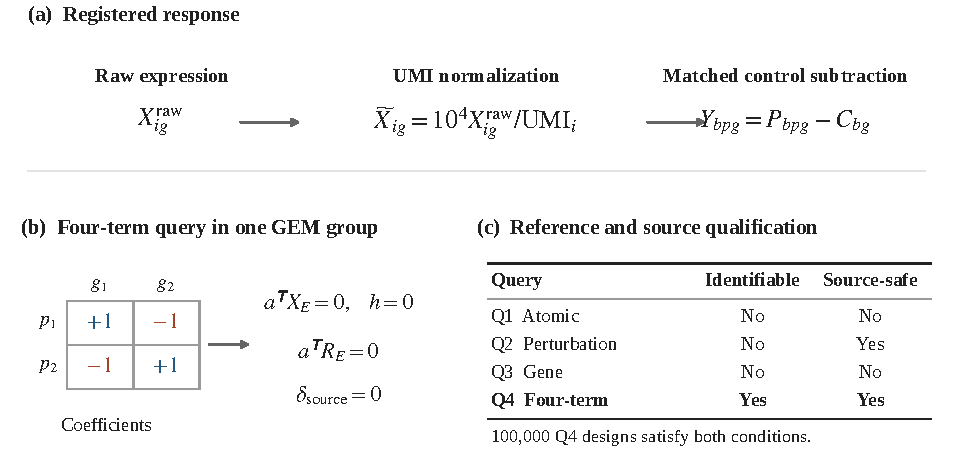
\includegraphics[width=\textwidth]{figures/figure_03.pdf}
\caption{\textbf{Reference and shared-control cancellation in registered Replogle Perturb-seq four-term query designs (RQ2).} Across $100{,}000$ four-cell interaction queries (Q4) constructed over the 256-gene panel ($310{,}385$ cells, $8{,}563$ genes, $48$ GEM groups, $97$ non-targeting control guides), alternating coefficients $(+1,-1,-1,+1)$ annihilate both the additive reference design ($a^\top X_E = 0$) and the equal-weight GEM shared-control map ($\delta_{\mathrm{source}} = 0$), preserving exact native-scale interaction contrasts without within-batch $z$-score distortion.}
\label{fig:replogle}
\end{figure}

Third, the Replogle K562 Perturb-seq resource~\cite{replogle2022perturbseq} ($310{,}385$ cell identities, $8{,}563$ genes, $48$ GEM groups, and $97$ non-targeting guide identities) provides a structural test of four-cell shared-source cancellation (Fig.~\ref{fig:replogle}). Under the registered equal-weight shared-control mapping on the frozen 256-gene panel, all \textbf{$100{,}000$ four-term query designs} satisfy reference estimability and declared-source cancellation, with no additional source-rank restriction. This agrees with the universal alternating-coefficient cancellation proved in Proposition~\ref{prop:fourcell}. The test concerns registered query geometry and metadata rather than newly extracted H5AD expression amplitudes. Supplementary Section~S13.2 derives how group-dependent standardization can change native-scale contrast values and signs. The $128$ native-identity two-GEM pools in Section~S13.3 further distinguish cancellation of GEM-by-gene from GEM-by-perturbation nuisance: a genuinely cross-GEM four-cell assignment cannot cancel both directly, whereas an eight-cell construction can combine two within-GEM contrasts.

\subsection{RQ3: Quotient target specification alters fixed-model rankings while persistence tests separate dataset stability}\label{subsec:result-eval}

We next evaluate how replacing ambient evaluation (\texttt{FULL}, $T=I$) with reference-resolved quotient evaluation (\texttt{ID}, $T=Q$) affects comparative model rankings across CTRPv2, GDSC2, GDSC1, and the symmetric-HPO retraining control (Fig.~\ref{fig:drug} and Table~\ref{tab:rq3_summary}).

\begin{figure}[t]
\centering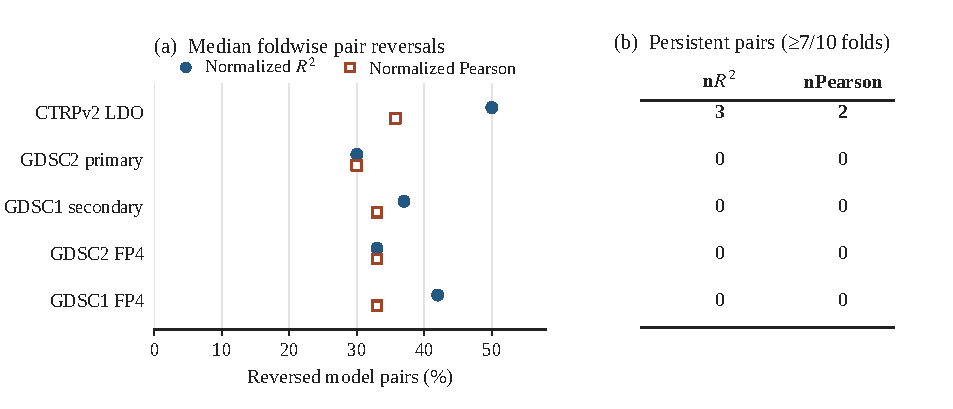
\includegraphics[width=\textwidth]{figures/figure_04.pdf}
\caption{\textbf{Fixed-prediction model comparisons and cross-fold preference reversals under \texttt{FULL} versus reference-resolved (\texttt{ID}) scoring (RQ3).} \textbf{(a)} Fold-wise pairwise ordering reversal fractions across the seven CTRPv2 leave-drug-out predictors (median $0.500$ under $\mathrm{n}R^2$ and $0.357$ under $\mathrm{n}r$) alongside external GDSC2, GDSC1, fingerprint-only common-support, and symmetric-HPO cohorts. \textbf{(b)} Directed pair--metric preference reversals meeting the prespecified $\ge 7/10$-fold persistence criterion: CTRPv2 exhibits $5$ persistent directed reversals across four non-naive model pairs (shifting the top mean $\mathrm{n}R^2$ predictor from \texttt{MultiOmicsNeuralNetwork} under \texttt{FULL} to \texttt{DIPK} under \texttt{ID}), whereas GDSC2 and GDSC1 exhibit substantial within-fold reversal rates ($0.30\text{--}0.37$) without a single pair reaching $\ge 7/10$-fold cross-split persistence. CTRPv2 uses registered model-specific supports; primary GDSC comparisons use common support.}
\label{fig:drug}
\end{figure}

On the primary CTRPv2 leave-drug-out benchmark ($7$ fixed predictors across $10$ frozen folds; $700$ archived metric fields verified with zero discrepancy by independent scoring replay), switching the evaluation target from \texttt{FULL} to \texttt{ID} reverses a \textbf{median fraction of $0.500$ of all model-pair orderings under $\mathrm{n}R^2$} and \textbf{$0.357$ under $\mathrm{n}r$} (Fig.~\ref{fig:drug}a). Across the ten folds, four non-naive model pairs generate \textbf{$5$ directed pair--metric preference reversals that persist in the exact same direction in at least $7$ of $10$ folds} ($3$ persistent reversals under $\mathrm{n}R^2$ and $2$ under $\mathrm{n}r$; Fig.~\ref{fig:drug}b). Most notably, the overall top-ranked predictor by arithmetic mean $\mathrm{n}R^2$ changes from \texttt{MultiOmicsNeuralNetwork} ($0.02347$) under \texttt{FULL} to \texttt{DIPK} ($0.02118$) under \texttt{ID}---without retraining any model or altering a single emitted prediction. As documented in Section~\ref{sec:design} and Supplementary Section~S4.6, because the archived CTRPv2 predictors retain model-specific post-merge observation supports, this seven-model reordering reflects target-component sensitivity under the registered model-specific-support protocol.

\begin{table}[t]
\centering\small\setstretch{1.08}
\caption{Benchmark ranking changes and cross-fold persistence under \paireval (RQ3). Reversals are directed pair--metric outcomes; the denominator for persistence is ten folds.}
\label{tab:rq3_summary}
\begin{tabularx}{\textwidth}{@{}L{0.22\textwidth}L{0.15\textwidth}L{0.13\textwidth}X@{}}
\toprule
Cohort and support & Median reversal n$R^2$/n$r$ & Persistent outcomes & Ranking and confirmation result\\\midrule
CTRPv2: 7 models, registered model-specific supports & $0.500/0.357$ & $5$ ($3/2$ by metric) & Highest mean n$R^2$ model changes from MultiOmicsNeuralNetwork to DIPK.\\
GDSC2: 6-model common support & $0.30/0.30$ & $0$ & Fold sensitivity exceeds $0.10$; the two-part confirmation criterion is not met.\\
GDSC1: 6-model common support & $0.37/0.33$ & $0$ & Fold-level ranking changes occur without seven-of-ten-fold directional persistence.\\
Fingerprint-only common support: GDSC2 / GDSC1 & $0.33/0.33$; $0.42/0.33$ & $0$ in both & Secondary support expansion preserves the absence of persistent outcomes.\\
Symmetric-HPO control: 560 jobs & Not summarized here & $1$ of $5$ historical outcomes & MultiOmicsNeuralNetwork--RandomForest n$R^2$ retains seven-of-ten-fold persistence in this new realization.\\\bottomrule
\end{tabularx}
\end{table}

The external pharmacogenomic confirmation studies on GDSC2 and GDSC1 (evaluated on the six-model common observation support; $420$ GDSC2 metric fields verified by scoring replay) reveal a critical distinction between \emph{within-fold scoring sensitivity} and \emph{cross-dataset preference persistence} (Table~\ref{tab:rq3_summary}). On GDSC2, switching from \texttt{FULL} to \texttt{ID} reverses a median of \textbf{$0.300$} of model pairs per fold under both $\mathrm{n}R^2$ and $\mathrm{n}r$---exceeding the prespecified $0.10$ fold-sensitivity threshold threefold---yet \textbf{$0$ directed pair--metric reversals reach the $\ge 7/10$-fold persistence threshold}. Consequently, the two-part prespecified GDSC2 confirmation criterion is not met. A parallel pattern holds in GDSC1, which exhibits median fold-level reversal fractions of \textbf{$0.370$} ($\mathrm{n}R^2$) and \textbf{$0.330$} ($\mathrm{n}r$) with zero persistent pairs, as well as in the fingerprint-only common-support sensitivity analysis. Furthermore, in our 560-job symmetric-HPO retraining control on CTRPv2, exactly \textbf{$1$ of the $5$ historical persistent pair--metric outcomes} (\texttt{MultiOmicsNeuralNetwork}--\texttt{RandomForest} under $\mathrm{n}R^2$) maintains $\ge 7/10$-fold persistence under newly trained weights. Finally, in the GDSC operator control comparing the exact pseudoinverse projector $Q$ against within-drug mean centering across two non-equivalent disconnected support topologies, both operators yield identical frozen model rankings (Supplementary Section~S4.7).

The frozen ENCODE splicing panel supplies a complementary target-definition example (Supplementary Section~S3.3). For the same three stored predictors, composite-only loss orders M2 (SVD-50) before M3 (additive-plus-LR-25) before M1 (additive), whereas unitwise-supported loss orders M3 before M2 before M1. This is a component-specific ordering on fixed predictions, separate from the drug-response fold-persistence protocol.

\section{Discussion}\label{sec:discussion}

\subsection{Why the comparison---not the imputed cell---is the natural unit of reuse}
The theoretical and empirical findings of this study converge on a single architectural principle for quantitative knowledge systems: \textbf{when a reference design is rank-deficient, the fundamental unit of verifiable knowledge reuse is the complete linear comparison $(a, h, z_{F_R}(a))$ rather than an imputed atomic cell}. As demonstrated in K562 APA ($26.50\%$) and ENCODE RBP splicing ($5.79\%$), thousands of orthogonal comparative dimensions are uniquely determined by the training reference even when their constituent individual design rows lie outside $\row(X_R)$. Standard atomic filtering discards this entire subspace, whereas matrix completion~\cite{mazumder2010softimpute,vo2026pica} assigns values using its declared reconstruction assumptions.

By pairing the coefficient vector $a$ with the completion witness $h^\top = a^\top X_E F_R$ and the four local verification identities in Proposition~\ref{prop:soundness}, \pairkg upgrades provenance tracking from passive metadata logging~\cite{w3c2013prov,sen2026provsql} to active algebraic certification. As shown in Section~\ref{subsec:complexity}, a downstream consumer receiving a \pairkg assertion does not need to trust a symbolic workflow tag or re-invert $X_R^\top X_R$; verifying $h^\top X_R = a^\top X_E$ and $a^\top R_E = h^\top R_R$ with the matrix--vector costs in Eq.~\eqref{eq:verifycost} locally confirms that the reported number is invariant to reference-null ambiguity and declared shared-source shifts. Our Replogle Perturb-seq analysis underscores the practical value of this algebraic contract: preserving the native additive scale allows balanced four-cell contrasts to cancel shared GEM controls universally across all generalized inverses (Proposition~\ref{prop:fourcell}), whereas routine within-GEM $z$-score preprocessing introduces group-dependent rescaling that can change the sign of an interaction contrast.

\subsection{Separating target-definition sensitivity from persistent model superiority}
In predictive benchmarking, \paireval demonstrates that ambient (\texttt{FULL}) and reference-resolved (\texttt{ID}) scores answer distinct scientific questions using the exact same predictions. In leave-drug-out pharmacogenomic evaluation, ambient scoring rewards a model both for predicting relative cell-line sensitivity profiles ($\operatorname{range}(Q)$) and for guessing the unseen drug's global mean potency offset ($\col(U)$). Stripping $\col(U)$ via $Q$ reverses $50.0\%$ of pairwise $\mathrm{n}R^2$ rankings in CTRPv2 and $30.0\%\text{--}37.0\%$ of rankings per fold in GDSC2 and GDSC1.

Equally important is the methodological lesson revealed by contrasting CTRPv2 (five persistent $\ge 7/10$-fold reversals) with GDSC2 and GDSC1 (zero persistent reversals despite $30\%\text{--}37\%$ per-fold reversal rates) and the 560-job symmetric-HPO control (one persistent reversal retained):
\begin{enumerate}
\item \emph{High per-fold reversal fractions ($30\%\text{--}50\%$)} show that the evaluated leaderboard scores are highly sensitive to whether reference-unresolved directions $\col(U)$ are included in the evaluation target.
\item \emph{Cross-fold and cross-cohort persistence checks} reveal that when competing models have closely matched relative-profile accuracy on a common observation support (or are retrained under symmetric HPO), the archived persistent preferences need not recur across resources or a new training realization.
\end{enumerate}
These findings give benchmark designers two connected decisions: first, explicitly specifying the evaluation target subspace ($Q$ vs. $I$) before interpreting leaderboard rankings; and second, coupling target projection with fold-persistence and common-support audits so that transient unresolved-space fluctuations are separated from persistent cross-fold preferences.

\subsection{Methodological scope, limitations, and future directions}
To guide responsible application of \method, several operational scope conditions should be kept in view:
\begin{itemize}
\item \emph{Algebraic admissibility versus statistical precision:} Passing the reference gate $a^\top U = 0$ certifies reference-null invariance; estimation variance is a separate quantity. As shown by our effective-resistance analysis in Supplementary Section~S11, sparse bridge edges in $X_R$ can yield estimable contrasts with high variance amplification $\|h\|_2^2$ (rising from median $0.07862$ on the original connected K562 support to $1.21967$ across a single-bridge cut, a median ratio of $15.53$), motivating joint admissibility and precision thresholds in future work.
\item \emph{Repeated mask exposures versus independent biological replication:} Cumulative subspace ranks across overlapping cross-validation masks ($150$ K562 masks, $20$ ENCODE masks, and $100{,}000$ Replogle Q4 designs) characterize structural design geometry on a fixed dataset rather than independent biological sample size (Supplementary Sections~S7.2 and S12).
\item \emph{Conditional replay of legacy archives:} When historical records omit native raw source tables or unregistered preprocessing operators, \pairkg witness verification certifies exact conditional reproducibility from the archived intermediate design ($2.3 \times 10^{-14}$ in K562 fold-0) rather than retrospective native-assay certification (Supplementary Sections~S6 and S10).
\item \emph{Support alignment in multi-model archives:} In legacy benchmarks where archived predictors retain distinct post-merge observation multisets (such as the seven-model CTRPv2 archive), cross-model ranking shifts reflect the joint effect of target projection $Q$ on each model's registered support; isolating pure target-component attribution requires enforcing a strict common observation support as implemented in our six-model GDSC1/GDSC2 protocol (Supplementary Section~S4.6).
\end{itemize}
Promising directions for future investigation include extending \method's linear quotient geometry to generalized linear models and exponential-family manifolds via local Fisher-information projections, integrating spectral effective-resistance bounds into automated active experimental design, and deploying self-verifying \pairkg witness records in federated multi-institutional biomedical knowledge graphs.

\section{Conclusion}\label{sec:conclusion}

PAIR connects quantitative knowledge compilation and model comparison through the information resolved by an experimental reference. PAIR-KG retains complete comparisons with completion-bound witnesses, reference and source checks, aggregation closure and source-refinement guarantees. PAIR-Eval uses the dual quotient space to decompose prediction error and determine when a model preference is invariant to reference completion. Across the evaluated resources, this representation retains 2,635 K562 and 56,395 ENCODE compound-only dimensions and supports shared-control cancellation for 100,000 Replogle designs. Fixed-prediction analyses show substantial ranking changes, while fold and cohort checks delimit their persistence. Together, the two interfaces make the reference, numerical meaning and decision target explicit when experimental evidence is reused in a knowledge-based system.

\section*{Data and code availability}
The public companion repository is available at \url{https://github.com/zhurunze44-hash/PAIR-IS-R9-reproducibility}, with the archived scoring-replay snapshot pinned at commit \href{https://github.com/zhurunze44-hash/PAIR-IS-R9-reproducibility/commit/496d1a3f3ea80009033891811ffa11ed9f7cf334}{496d1a3f3ea8}. This pinned software snapshot provides constructed exact-rational checks, scorer-replay programs, and evidence inventories. The current manuscript sources are supplied separately; large frozen prediction arrays and complete historical producer inputs are not all redistributed. Resource-specific reproduction scopes are detailed in Supplementary Sections~S6 and S15.

\Needspace{6\baselineskip}
\section*{CRediT authorship contribution statement}
\AuthorContributions
\section*{Funding}
\FundingStatement
\section*{Declaration of competing interest}
\CompetingInterests
\section*{Declaration of generative AI and AI-assisted technologies in manuscript preparation}
During manuscript preparation, the authors used Google Gemini (model version not retained) and OpenAI ChatGPT with Codex assistance for editorial revision, translation, LaTeX preparation, and deterministic figure-code support. The authors reviewed and edited the content and take responsibility for the publication. Computational and figure assistance is described in Supplementary Section~S6.4.

\begingroup\small\setstretch{1.0}\setlength{\bibsep}{0pt}
\bibliographystyle{unsrtnat}
\bibliography{references}
\endgroup
\end{document}
